%%%% CS 224N: Assignment #1 %%%%
%\documentclass[fleqn,10pt]{article}
%\usepackage{simplemargins}
%\setallmargins{1.0in}
\documentclass[10pt,reqno]{amsart}
\usepackage{amsmath}
\usepackage{amssymb}
\usepackage{amsthm}
\usepackage{bm}
\usepackage{enumitem}
\usepackage{graphicx}
\usepackage[paper=letterpaper,margin=0.75in]{geometry}
\usepackage[all]{xy}

%% Define header
\begin{document}
\title{CS224n: Natural Language Processing with Deep Learning\\Assignment \#1}
\author{Anthony Ho}
\maketitle


%% Define shortcuts
\newcommand{\f}{\frac}
\newcommand{\pd}[1]{\frac{\partial}{\partial #1}}
\newcommand{\pdd}[2]{\frac{\partial #1}{\partial #2}}
\newcommand{\softmax}{\text{softmax}}


%% Set up numbering environment
\renewcommand{\labelenumi}{\arabic{enumi}.}
\begin{enumerate}[topsep=0pt,itemsep=3ex,partopsep=1ex,parsep=1ex]


%% Question 1
\item
  \begin{enumerate}[itemsep=2ex]
  %% Question 1(a)
  \item
    For any input vector $\bm{x}$ and any constant $c$,
    \begin{align}
      \softmax(\bm{x} + c)_i
      &= \f{e^{x_i + c}}{\sum_j e^{x_j + c}} \nonumber \\
      &= \f{e^c e^{x_i}}{\sum_j e^c e^{x_j}} \nonumber \\
      &= \f{e^c e^{x_i}}{e^c \sum_j e^{x_j}} \nonumber \\
      &= \f{e^{x_i}}{\sum_j e^{x_j}} \nonumber \\
      &= \softmax(\bm{x})_i \label{1a}
    \end{align}
    Since (\ref{1a}) is true for any arbitrary element $i$,
    we can conclude that:
    \begin{equation*}
      \softmax(\bm{x}) = \softmax(\bm{x} + c)
    \end{equation*}
    
  %% Question 1(b)
  \item Please see the coding portion of the assignment.
  \end{enumerate}


%% Question 2
\item
  \begin{enumerate}[itemsep=2ex]
  %% Question 2(a)
  \item 
    First, we can rearrange the definition of the sigmoid function to obtain:
    \begin{align*}
      e^{-x} = \f{1}{\sigma(x)} - 1
    \end{align*}
    Now we can derive the gradient of the sigmoid function w.r.t. $x$,
    assuming $x$ is a scalar. 
    \begin{align*}
      \pdd{\sigma(x)}{x}
      &= \pd{x} \f{1}{1 + e^{-x}} \\
      &= \f{-1}{(1 + e^{-x})^2} \left( - e^{-x} \right) \\
      &= \f{1}{(1 + e^{-x})^2} \left( e^{-x} \right) \\
      &= \left( \sigma(x) \right)^2 \left( \f{1}{\sigma(x)} - 1 \right) \\
      &= \sigma(x) \left( 1 - \sigma(x) \right)
    \end{align*}

  %% Question 2(b)
  \item
    First, let's consider the fact that $\bm{y}$ is the one-hot label vector, i.e.
    \begin{equation*}
      y_i = 
      \begin{cases}
        1, & \text{if}\ i=k \\
        0, & \text{otherwise}
      \end{cases}
    \end{equation*}
    where $k$ is the index of the true label. 
    
    Therefore, we can simplify the cross entropy function as:
    \begin{equation*}
      \text{CE}(\bm{y}, \bm{\hat{y}})
        = - \sum_i y_i \log(\hat{y}_i)
        = - \log(\hat{y}_k)
    \end{equation*}

    To derive the gradient w.r.t the inputs of a softmax function when cross entropy loss
    is used for evaluation, let's consider its individual elements:
    \begin{align}
      \pd{\theta_i} \text{CE}(\bm{y}, \bm{\hat{y}})
      &= \pd{\theta_i} \left[ - \log(\hat{y}_k) \right] \nonumber \\
      &= \pd{\theta_i} \left[ - \log(\f{e^{\theta_k}}{\sum_j e^{\theta_j}}) \right] \nonumber \\
      &= \pd{\theta_i} \left[ -\theta_k + \log \sum_j e^{\theta_j} \right] \nonumber \\
      &= - \pdd{\theta_k}{\theta_i} + \f{\sum_j e^{\theta_j} \pdd{\theta_j}{\theta_i}}{\sum_j e^{\theta_j}} \label{2b}
    \end{align}

    By noting that:
    \begin{equation*}
      \pdd{\theta_j}{\theta_i} = 
      \begin{cases}
        1, & \text{if}\ i=j \\
        0, & \text{otherwise}
      \end{cases}
    \end{equation*}

    We can simpify (\ref{2b}) as:
    \begin{equation*}
      \pd{\theta_i} \text{CE}(\bm{y}, \bm{\hat{y}})
      = - y_i + \f{e^{\theta_i}}{\sum_j e^{\theta_j}} 
      = - y_i + \hat{y}_i 
    \end{equation*}

    Thus, the gradient w.r.t the inputs of a softmax function when cross entropy loss
    is used for evaluation is:
    \begin{equation*}
      \pd{\bm{\theta}} \text{CE}(\bm{y}, \bm{\hat{y}}) = \bm{\hat{y}} - \bm{y}
    \end{equation*}

  %% Question 2(c)
  \item
    Let's denote:
    \begin{align*}
      \bm{\theta_1} &= \bm{x W_1} + \bm{b_1} \\
      \bm{\theta_2} &= \bm{h W_2} + \bm{b_2}
    \end{align*}
    
    By applying chain rule, we can rewrite the gradient as:
    \begin{equation*}
      \pdd{J}{\bm{x}}
      = \pdd{\text{CE}(\bm{y}, \bm{\hat{y}})}{\bm{x}}
      = \pdd{\text{CE}(\bm{y}, \bm{\hat{y}})}{\bm{\theta_2}} \pdd{\bm{\theta_2}}{\bm{h}} \pdd{\bm{h}}{\bm{\theta_1}} \pdd{\bm{\theta_1}}{\bm{x}}
    \end{equation*}
    
    The first component is simply the result of part (b):
    \begin{equation*}
      \pdd{\text{CE}(\bm{y}, \bm{\hat{y}})}{\bm{\theta_2}} = \bm{\hat{y}} - \bm{y}
    \end{equation*}
    
    The second component is:
    \begin{equation*}
      \pdd{\bm{\theta_2}}{\bm{h}} = \pd{\bm{h}} \left( \bm{h W_2} + \bm{b_2} \right) = \bm{W_2}^\top
    \end{equation*}

    The third component is a $H \times H$ matrix
    and can be computed by examining its individual elements:
    \begin{equation*}
      \left( \pdd{\bm{h}}{\bm{\theta_1}} \right)_{ij}
      = \left( \pdd{\sigma(\bm{\theta_1})}{\bm{\theta_1}} \right)_{ij} 
      = \pdd{(\sigma(\bm{\theta_1}))_i}{{\theta_1}_j}
      = \pdd{\sigma({\theta_1}_i)}{{\theta_1}_j} = 
      \begin{cases}
        \sigma'({\theta_1}_i), & \text{if}\ i=j \\
        0, & \text{otherwise}
      \end{cases}
    \end{equation*}
    where $\sigma'({\theta_1}_i) = \sigma({\theta_1}_i) \left( 1 - \sigma({\theta_1}_i) \right)$
    is the sigmoid gradient as shown in part (a).

    Thus, we can define: 
    \begin{equation*}
      \pdd{\bm{h}}{\bm{\theta_1}} = \bm{S}(\bm{\theta_1})
    \end{equation*}
    where $\bm{S}$ denotes a $H \times H$ diagonal matrix where 
    the diagonal elements are $\sigma'(\theta_i)$ for $i = 1, \cdots, H$.

    The fourth component is similar to the second component:
    \begin{equation*}
      \pdd{\bm{\theta_1}}{\bm{x}} = \pd{\bm{x}} \left( \bm{x W_1} + \bm{b_1} \right) = \bm{W_1}^\top
    \end{equation*}

    Therefore, the the gradient with respect to the inputs $\bm{x}$ to an one-hidden-layer neural network is:
    \begin{align*}
      \pdd{J}{\bm{x}}
      &= \pdd{\text{CE}(\bm{y}, \bm{\hat{y}})}{\bm{\theta_2}} \pdd{\bm{\theta_2}}{\bm{h}} \pdd{\bm{h}}{\bm{\theta_1}} \pdd{\bm{\theta_1}}{\bm{x}} \\
      &= \left( \bm{\hat{y}} - \bm{y} \right) \bm{W_2}^\top \bm{S}(\bm{\theta_1}) \bm{W_1}^\top \\
      &= \left( \bm{\hat{y}} - \bm{y} \right) \bm{W_2}^\top \bm{S}(\bm{x W_1} + \bm{b_1}) \bm{W_1}^\top
    \end{align*}

    Or, equivalently:
    \begin{equation*}
      \pdd{J}{\bm{x}} 
      = \left( \bm{\hat{y}} - \bm{y} \right) \bm{W_2}^\top 
      \circ \sigma(\bm{x W_1} + \bm{b_1}) \circ ( 1 - \sigma(\bm{x W_1} + \bm{b_1}) ) \bm{W_1}^\top
    \end{equation*}
    where $\circ$ denotes the Hadamard product of two vectors. 
  %% Question 2(d)
  \item
    The dimensions of the weights and biases are as follows:
    \vspace{1mm}
    \begin{center}
      \begin{tabular}{|c|c|}
        \hline
        Parameter & Dimension \\
        \hline
        $W_1$ & $D_x \times H$ \\
        $b_1$ & $1 \times H$ \\
        $W_2$ & $H \times D_y$ \\
        $b_2$ & $1 \times D_y$ \\
        \hline
      \end{tabular}
    \end{center}
    \vspace{1mm}
    Therefore, the number of parameters in this neural network is:
    \begin{equation*}
      \text{\# parameters} = D_x H + H + H D_y + D_y = (D_x + 1) H + D_y (H + 1)
    \end{equation*}

  %% Question 2(e)
  \item Please see the coding portion of the assignment.
  %% Question 2(f)
  \item Please see the coding portion of the assignment.
  %% Question 2(g)
  \item Please see the coding portion of the assignment.
  \end{enumerate}


%% Question 3
\item
  \begin{enumerate}[itemsep=2ex]
  %% Question 3(a)
  \item
    Let's denote:
    \begin{align*}
      \theta_w &= \bm{u}_w^\top \bm{v}_c \\
      \bm{\theta} &= \bm{U}^\top \bm{v}_c
    \end{align*}
    where $\theta_w$ is a scalar,
    $\bm{u}_w$ and $\bm{v}_c$ are column vectors of dimensions $N \times 1$,
    $\bm{\theta}$ is a column vector of dimension $V \times 1$, 
    and $\bm{U} = [\bm{u}_1, \bm{u}_2, \cdots, \bm{u}_V]$ is a matrix of dimension $N \times V$.

    The softmax predictions for every word can then be written as:
    \begin{equation*}
      \bm{\hat{y}} = \f{\exp(\bm{U}^\top \bm{v}_c)}{\sum_{w=1}^{V} \exp(\bm{u}_w^\top \bm{v}_c)}
      = \f{\exp(\bm{\theta})}{\sum_{w=1}^{V} \exp(\theta_w)}
    \end{equation*}
    where $\bm{\hat{y}}$ is a column vector of softmax predictions for every word of dimension $V \times 1$.

    By using chain rule and the result of 2(b), the gradient of the cross entropy cost w.r.t. $\bm{v}_c$ 
    can be derived as:
    \begin{align*}
      \pd{\bm{v}_c} J_\text{softmax--CE}
      &= \pdd{\bm{\theta}}{\bm{v}_c} \pdd{J}{\bm{\theta}} \\
      &= \pdd{\bm{U}^\top \bm{v}_c}{\bm{v}_c} \pdd{\text{CE}(\bm{y}, \bm{\hat{y}})}{\bm{\theta}} \\
      &= \bm{U} \left( \bm{\hat{y}} - \bm{y} \right)
    \end{align*}
    where $\bm{y}$ is a column vector of expected word of dimension $V \times 1$.
  %% Question 3(b)
  \item
    As in the previous part, we can apply chain rule and the result of 2(b):
    \begin{align}
      \pd{\bm{u}_k} J_\text{softmax--CE}
      &= \pdd{\bm{\theta}}{\bm{u}_k} \pdd{J}{\bm{\theta}} \nonumber \\
      &= \pdd{\bm{U}^\top \bm{v}_c}{\bm{u}_k} \pdd{\text{CE}(\bm{y}, \bm{\hat{y}})}{\bm{\theta}} \nonumber \\
      &= \pdd{\bm{U}^\top \bm{v}_c}{\bm{u}_k} \left( \bm{\hat{y}} - \bm{y} \right) \label{3b}
    \end{align}
    
    Rewriting matrix multiplication in (\ref{3b}) explicitly:
    \begin{align*}
      \pd{\bm{u}_k} J_\text{softmax--CE}
      &= \sum_j^V \left( \bm{\hat{y}} - \bm{y} \right)_j \left( \pdd{\bm{U}^\top \bm{v}_c}{\bm{u}_k} \right)_{\cdot j} \\
      &= \sum_j^V \left( \hat{y}_j - y_j \right) \left( \pdd{\bm{U}^\top \bm{v}_c}{\bm{u}_k} \right)_{\cdot j} 
    \end{align*}
    where $\left( \pdd{\bm{U}^\top \bm{v}_c}{\bm{u}_k} \right)_{\cdot j}$ is the $j$-th column of 
    $\pdd{\bm{U}^\top \bm{v}_c}{\bm{u}_k}$ which is a $N \times V$ matrix.
    It can be simplified to:
    \begin{equation*}
      \left( \pdd{\bm{U}^\top \bm{v}_c}{\bm{u}_k} \right)_{\cdot j} =
      \begin{cases}
        \bm{v}_c, & \text{if}\ j=k \\
        0, & \text{otherwise}
      \end{cases}
    \end{equation*}

    Therefore,the gradient can be simplified to:
    \begin{align*}
      \pd{\bm{u}_k} J_\text{softmax--CE} 
      &= \left( \hat{y}_k - y_k \right) \bm{v}_c
    \end{align*}

    Specifically,
    \begin{equation*}
      \pd{\bm{u}_k} J_\text{softmax--CE} =
      \begin{cases}
        \left( \hat{y}_k - 1 \right) \bm{v}_c, & \text{if}\ k=o \\
        \hat{y}_k \bm{v}_c, & \text{otherwise}
      \end{cases}
    \end{equation*}    

  %% Question 3(c)
  \item
    Let's denote:
    \begin{align*}
      \theta_o &= \bm{u}_o^\top \bm{v}_c \\
      \theta_k &= - \bm{u}_k^\top \bm{v}_c 
    \end{align*}

    The gradient of the negative sampling loss w.r.t. $\bm{v}_c$ is:
    \begin{align*}
      \pd{\bm{v}_c} J_\text{neg−-sample}
      &= \pd{\bm{v}_c} \left[ -\log(\sigma(\bm{u}_o^\top \bm{v}_c)) - \sum_{k=1}^K \log(\sigma(-\bm{u}_k^\top \bm{v}_c)) \right] \\
      &= \pd{\bm{v}_c} \left[ -\log(\sigma(\theta_o)) - \sum_{k=1}^K \log(\sigma(\theta_k)) \right] \\
      &= - \f{1}{\sigma(\theta_o)} \pdd{\sigma(\theta_o)}{\theta_o} \pdd{\theta_o}{\bm{v}_c} 
         - \sum_{k=1}^K \f{1}{\sigma(\theta_k)} \pdd{\sigma(\theta_k)}{\theta_k} \pdd{\theta_k}{\bm{v}_c} \\
      &= - \f{1}{\sigma(\theta_o)} \sigma(\theta_o) (1 - \sigma(\theta_o)) \pdd{\theta_o}{\bm{v}_c} 
         - \sum_{k=1}^K \f{1}{\sigma(\theta_k)} \sigma(\theta_k) (1 - \sigma(\theta_k)) \pdd{\theta_k}{\bm{v}_c} \\
      &= (\sigma(\bm{u}_o^\top \bm{v}_c) - 1)  \pdd{\bm{u}_o^\top \bm{v}_c}{\bm{v}_c} 
         + \sum_{k=1}^K (\sigma(-\bm{u}_k^\top \bm{v}_c) - 1) \pdd{(-\bm{u}_k^\top \bm{v}_c)}{\bm{v}_c} \\
      &= (\sigma(\bm{u}_o^\top \bm{v}_c) - 1) \bm{u}_o - \sum_{k=1}^K (\sigma(-\bm{u}_k^\top \bm{v}_c) - 1) \bm{u}_k
    \end{align*}

    Similarly, the gradient of the negative sampling loss w.r.t. $\bm{u}_o$ is:
    \begin{align*}
      \pd{\bm{u}_o} J_\text{neg−-sample}
      &= (\sigma(\bm{u}_o^\top \bm{v}_c) - 1)  \pdd{\bm{u}_o^\top \bm{v}_c}{\bm{u}_o} 
         + \sum_{k=1}^K (\sigma(-\bm{u}_k^\top \bm{v}_c) - 1) \pdd{(-\bm{u}_k^\top \bm{v}_c)}{\bm{u}_o} \\
      &= (\sigma(\bm{u}_o^\top \bm{v}_c) - 1) \bm{v}_c
    \end{align*}

    And the gradient of the negative sampling loss w.r.t. $\bm{u}_k$ is
    (changing summation indices from $k$ to $j$ to avoid confusion):
    \begin{align*}
      \pd{\bm{u}_k} J_\text{neg−-sample}
      &= (\sigma(\bm{u}_o^\top \bm{v}_c) - 1)  \pdd{\bm{u}_o^\top \bm{v}_c}{\bm{u}_k} 
         + \sum_{j=1}^K (\sigma(-\bm{u}_j^\top \bm{v}_c) - 1) \pdd{(-\bm{u}_j^\top \bm{v}_c)}{\bm{u}_k} \\
      &= (1 - \sigma(-\bm{u}_k^\top \bm{v}_c)) \bm{v}_c
    \end{align*}

    This cost function is much more efficient to compute than the softmax-CE loss 
    because the computation of $\pdd{J}{\bm{v}_c}$ for softmax-CE loss scales as $V$
    while the computation of $\pdd{J}{\bm{v}_c}$ for negative sampling loss scales as $K$, 
    resulting in a speed-up ratio of $K/V$,
    which could make a huge difference if one has a big vocabulary.

  %% Question 3(d)
  \item
    For skip-gram, the cost for a context centered around c is:
    \begin{equation*}
      J_\text{skip-gram}(w_{t-m},\cdots,w_{t+m})
      = \sum_{-m \leq j \leq m, j \neq 0} F(w_{t+j}, \bm{v}_c)
    \end{equation*}
    where
    \begin{equation*}
      F(o, \bm{v}_c) = 
      \begin{cases}
        J_\text{softmax--CE}(o, \bm{v}_c, \cdots) = \text{CE}(\bm{y}, \bm{\hat{y}}) = - \displaystyle\sum_i^V y_i \log(\hat{y}_i), & \text{for softmax--CE loss} \\
        J_\text{neg−-sample}(o, \bm{v}_c, \cdots) = -\log(\sigma(\bm{u}_o^\top \bm{v}_c)) - \displaystyle\sum_{k=1}^K \log(\sigma(-\bm{u}_k^\top \bm{v}_c)), & \text{for negative sampling loss}
      \end{cases}
    \end{equation*}

    Therefore, the gradients w.r.t. the word vectors for the skip-gram model are:
    \begin{align*}
      \pd{\bm{v}_k} J_\text{skip-gram}(w_{t-m},\cdots,w_{t+m}) &= 
      \begin{cases}
        \displaystyle\sum_{-m \leq j \leq m, j \neq 0} \pdd{F(w_{t+j}, \bm{v}_c)}{\bm{v}_c}, & \text{if}\ k = c \\
        \qquad\qquad\qquad 0, & \text{otherwise}
      \end{cases}\\
      \pd{\bm{u}_k} J_\text{skip-gram}(w_{t-m},\cdots,w_{t+m}) 
      &= \sum_{-m \leq j \leq m, j \neq 0} \pdd{F(w_{t+j}, \bm{v}_c)}{\bm{u}_k} 
    \end{align*}

    For CBOW, the cost is:
    \begin{equation*}
      J_\text{CBOW}(w_{t-m},\cdots,w_{t+m}) = F(w_t, \bm{\hat{v}})
    \end{equation*}
    where
    \begin{equation*}
      \bm{\hat{v}} = \sum_{-m \leq j \leq m, j \neq 0} \bm{v}_{w_{t+j}}
    \end{equation*}

    Therefore, the gradients w.r.t. the word vectors for the CBOW model are:
    \begin{align*}
      \pd{\bm{v}_k} J_\text{CBOW}(w_{t-m},\cdots,w_{t+m}) &= 
      \begin{cases}
        \displaystyle\pdd{F(w_t, \bm{\hat{v}})}{\bm{\hat{v}}} \pdd{\bm{\hat{v}}}{\bm{v}_k} 
        = \displaystyle\pdd{F(w_t, \bm{\hat{v}})}{\bm{\hat{v}}} , & \text{if}\ t-m \leq k \leq t+m\ \text{and}\ k \neq t\\
        \qquad\qquad\qquad 0, & \text{otherwise}
      \end{cases}\\
      \pd{\bm{u}_k} J_\text{CBOW}(w_{t-m},\cdots,w_{t+m}) 
      &= \pdd{F(w_t, \bm{\hat{v}})}{\bm{u}_k} 
    \end{align*}
    
  %% Question 3(e)
  \item Please see the coding portion of the assignment.
  %% Question 3(f)
  \item Please see the coding portion of the assignment.
  %% Question 3(g)
    \begin{figure}[h!]
      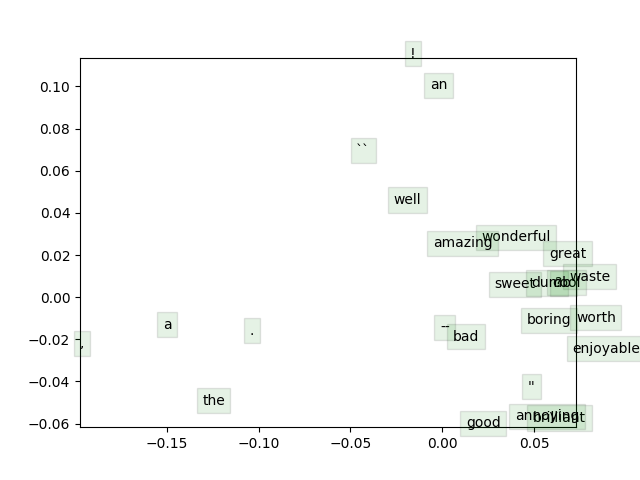
\includegraphics[width=0.75\textwidth]{../code/q3_word_vectors.png}
      \caption{Visualization for the word vectors.}
      \label{fig1}
    \end{figure}
  \item
    Figure \ref{fig1} shows the visualization for the word vectors. 
    First we can immediately notice it that all the adjectives cluster together, 
    while articles and punctuations scatter around. 
    Also, we observe that many pairs of adjectives that have opposite meanings 
    form vectors that point to approximately the same direction, such as 
    bad$\,\to\,$good, 
    boring$\,\to\,$enjoyable,
    dumb$\,\to\,$brilliant, and
    waste$\,\to\,$worth.
  %% Question 3(h)
  \item
  \end{enumerate}


%% Question 4
\item
  \begin{enumerate}[itemsep=2ex]
  %% Question 4(a)
  \item Please see the coding portion of the assignment.
  %% Question 4(b)
  \item Regularization helps prevent overfitting and reduce model complexity,
    which would help increase prediction and generalization power to new datasets.
  %% Question 4(c)
  \item Please see the coding portion of the assignment.
  %% Question 4(d)
  \item
  %% Question 4(e)
  \item
  %% Question 4(f)
  \item
  %% Question 4(g)
  \item
  \end{enumerate}

\end{enumerate}
\end{document}
